\documentclass[a4paper]{article}
\usepackage{lab}
\usepackage{enumitem}
\usepackage{steinmetz}
\usepackage{amsmath}
\usepackage{hyperref}
\hypersetup{
	colorlinks=true,
	urlcolor=blue,
	pdfnewwindow=true
}

\begin{document}

\begin{titlepage}
	\thispagestyle{fancy} %For the left header
	\rhead{}
	\chead{}
	\lhead{Project \#1}
	\rfoot{}
	\cfoot{}
	\lfoot{}
	\renewcommand{\headrulewidth}{0pt} %Removes horizontal line
	\begin{center}
		\vspace*{1cm}
		
		\Large\textbf{University of North Carolina at Charlotte \\[1pt]
			Department of Electrical and Computer Engineering} \\[2pt]
		\vspace*{1cm}
		
		\noindent\rule{15cm}{0.4pt}
		\vfill
		\LARGE\textbf{Aircraft-Detection Radar - ECGR 5121} \\ [1pt]
		\vspace{1cm}
		Author: Miguel Aviles \\
		Lab Partner: None	\\
		Date: 10/18/2026 \\
		\vspace{1.5cm}
		
		\vfill
		\vfill
	\end{center}
\end{titlepage}

\section{Objectives}
	Design a $f = 10$ GHz monostatic radar to detect an aircraft at a range of $R_0 = 20$ km. The aircraft radar cross-section (RCS) varies with the azimuthal aspect angle relative to the radar. The below objectives provide a step-step framework for developing an applicable antenna for this application:
	\begin{enumerate}
		\item Plot the supplied aircraft RCS in dBsm versus azimuthal aspect angle using Cartesian coordinates.
		\item Plot the supplied aircraft RCS in dBsm versus azimuthal aspect angle using polar coordinates.
		\item Calculate and plot the required gain $G$ in dBi versus aircraft azimuthal aspect angle.
		\item Determine the minimum antenna gain $G$ required to detect the aircraft for at least 90 percent of the supplied aspect angles.
		\item Utilize the required gain derived above to determine the required reflector diameter $D$, the reflector radius $a$, and the focal length $f_p$ such that $\frac{f_p}{D} < 0.4$.
		\item Design a parabolic reflector antenna with parameters such that the required gain $G$ is achieved utilizing the MATLAB Antenna Toolbox.
	\end{enumerate}

\section{Theoretical Background}
	\subsection{Radar Wavelength and Frequency Relationship}
	The operating frequency dictates the physical size of our antenna, since the wavelength is directly related to the frequency through the phase velocity $v_p$ of the medium, which in our case will constitute free-space phase velocity, also known as the speed of light $c$. The expression for operating wavelength is given below: 
	\begin{equation}
		\lambda = \frac{c}{f}
	\end{equation}
	The fundamental scaling of our antenna design will depend on the operating wavelength calculated, which depends on the operating frequency chosen. The expression above indicates that higher frequencies tend to lower the wavelength of operation, which therefore lowers the size of the antenna needed, which in most applications is ideal.
	
	\subsection{The Monostatic Radar Equation}
	The core equation which defines all of the parameters needed for designing an effective antenna is the Monostatic Radar Equation, which is given below:
	\begin{equation}
		P_r = \frac{P_t G^2 \lambda^2 \sigma}{(4\pi)^3 R^4}
	\end{equation}
	Where:
	\begin{itemize}
		\item $P_r$ = Received Back-scatter Power (W)
		\item $P_t$ = Peak Transmitted Power (W)
		\item $G$ = Antenna Gain (dimensionless linear)
		\item $\lambda$ = Operating Wavelength (m)
		\item $\sigma$ = Target Radar Cross-Section ($m^2$)
		\item $R$ = Distance from target (m)
	\end{itemize}
	The received back-scatter power $P_r$ from a target at a range $R$ depends on the transmitted power $P_t$, the antenna gain $G$, the operating wavelength $\lambda$, and the target radar cross-section $\sigma$. The target radar cross-section is also known as the RCS, which is the value which varies with azimuthal aspect angle relative to the radar. 
	
	To ensure the radar system can successfully detect an aircraft at the maximum design range $R_0$, the receieved power $P_r$ must equal to exceed a minimum detectable threshold. Therefore, assuming the operating wavelength $\lambda$, the transmitted power $P_t$ and the RCS over a given azimuthal angle range are known, then a required antenna gain can be derived from the Monostatic Radar Equation. The expression for the required gain is given below:
	\begin{equation}
		G_{req} = \sqrt{\frac{P_{rmin} (4\pi)^3 R_0^4}{P_t \lambda^2 \sigma}}
	\end{equation}
	The antenna gain $G$ is typically expressed as decibels relative to an isotropic antenna (dBi) on a logarithmic scale. The conversion from linear to logarithmic gain is given below:
	\begin{equation}
		G_{req (dBi)} = 10\log(G_{req})
	\end{equation}
	In general, it is difficult and unnecessary to define our antenna gain for covering 100 percent of potential aspect angles. Therefore, choosing a reasonable threshold (such as 90 percent) will minimize the gain requirements of our antenna while working nearly as effectively.
	
	\subsection{Parabolic Reflector Antenna Theory}
	The parabolic reflector topology provides high directivity (and therefore high gain), which is perfect for our application. A parabolic reflector focuses EM waves produced by the point-source feed antenna into highly directive, planar EM waves. The maximum gain of a parabolic reflector antenna is given by the expression below:
	\begin{equation}
		G = \eta_{ap} (\frac{\pi D}{\lambda})^2
	\end{equation}
	Where:
	\begin{itemize}
		\item $G$ = Maximum Antenna Gain (dimensionless linear)
		\item $\eta_{ap}$ = Aperture Efficiency (unitless)
		\item $D$ = Physical Diameter of the reflector (m)
		\item $\lambda$ = Operating Wavelength (m)
	\end{itemize}
	From the above expression it is clear that high gain $G$ is achieved by increasing the reflector diameter $D$ relative to the operating wavelength $\lambda$.
	
	The aperture efficiency $\eta_{ap}$ is the ratio of effective aperture area $A_e$ to the physical aperture area $A_{phys}$. This quantity effectively accounts for various losses due to surface roughness, feed blockage and other non-idealities. 
	
	The required gain is calculated above utilizing the Equation 3, and therefore Equation 5 is rearranged to find the physical diameter of our parabolic reflector antenna, assuming a known aperature efficiency factor. The rearranged expression is given below:
	\begin{equation}
		D = \frac{\lambda}{\pi} \sqrt{\frac{G}{\eta_{ap}}}
	\end{equation}
	The radius of the reflector antenna is simply $a = \frac{D}{2}$. The required antenna gain $G$ is converted from logarithmic to linear through the below expression:
	\begin{equation}
		G_{req (linear)} = 10^{\frac{G_{req (dBi)}}{10}}
	\end{equation}
	The focal length (distance from feed antenna to the center of the reflector) is another important design parameter for parabolic antennas. In our application, the focal ratio is given as $\frac{f_p}{D} < 0.4$, which defines a deep reflector antenna, since the outer edge of the dish curves inward much more sharply, reducing the influence of outside noise. 
	
	Combining all of these parameters together, an appropriate parabolic reflector antenna which meets the required gain $G$ set by the Monostatic Radar equation can be designed using tools such as MATLAB's Antenna Toolbox easily.
	
\section{Simulation Method}
	To begin, MATLAB is utilized in order to calculate all relevant parameters and plots. View the references section to access the MATLAB code and RCS data through Github. After setup, we define our initial parameters and conditions below:
	\begin{itemize}
		\item $P_t$ = $1000$W
		\item $f$ = $10$GHz
		\item $R_0$ = $20$km
		\item $P_{rmin}$ = $1\cdot10^{-13}$W
		\item $\eta_{ap}$ = $0.34$
		\item $\frac{f_p}{D} < 0.4$
	\end{itemize}
    The RCS (dBsm) vs. Azimuthal Aspect Angle (degrees) data is plotted in both Cartesian and Polar coordinates. The larger the RCS, the lower the required gain for that given angle. Therefore, when the gain vs. aspect angle is plotted, the high RCS points will become the lower required gain regions. The plots are shown below:
    \begin{figure}[H]
    	\begin{center}
    		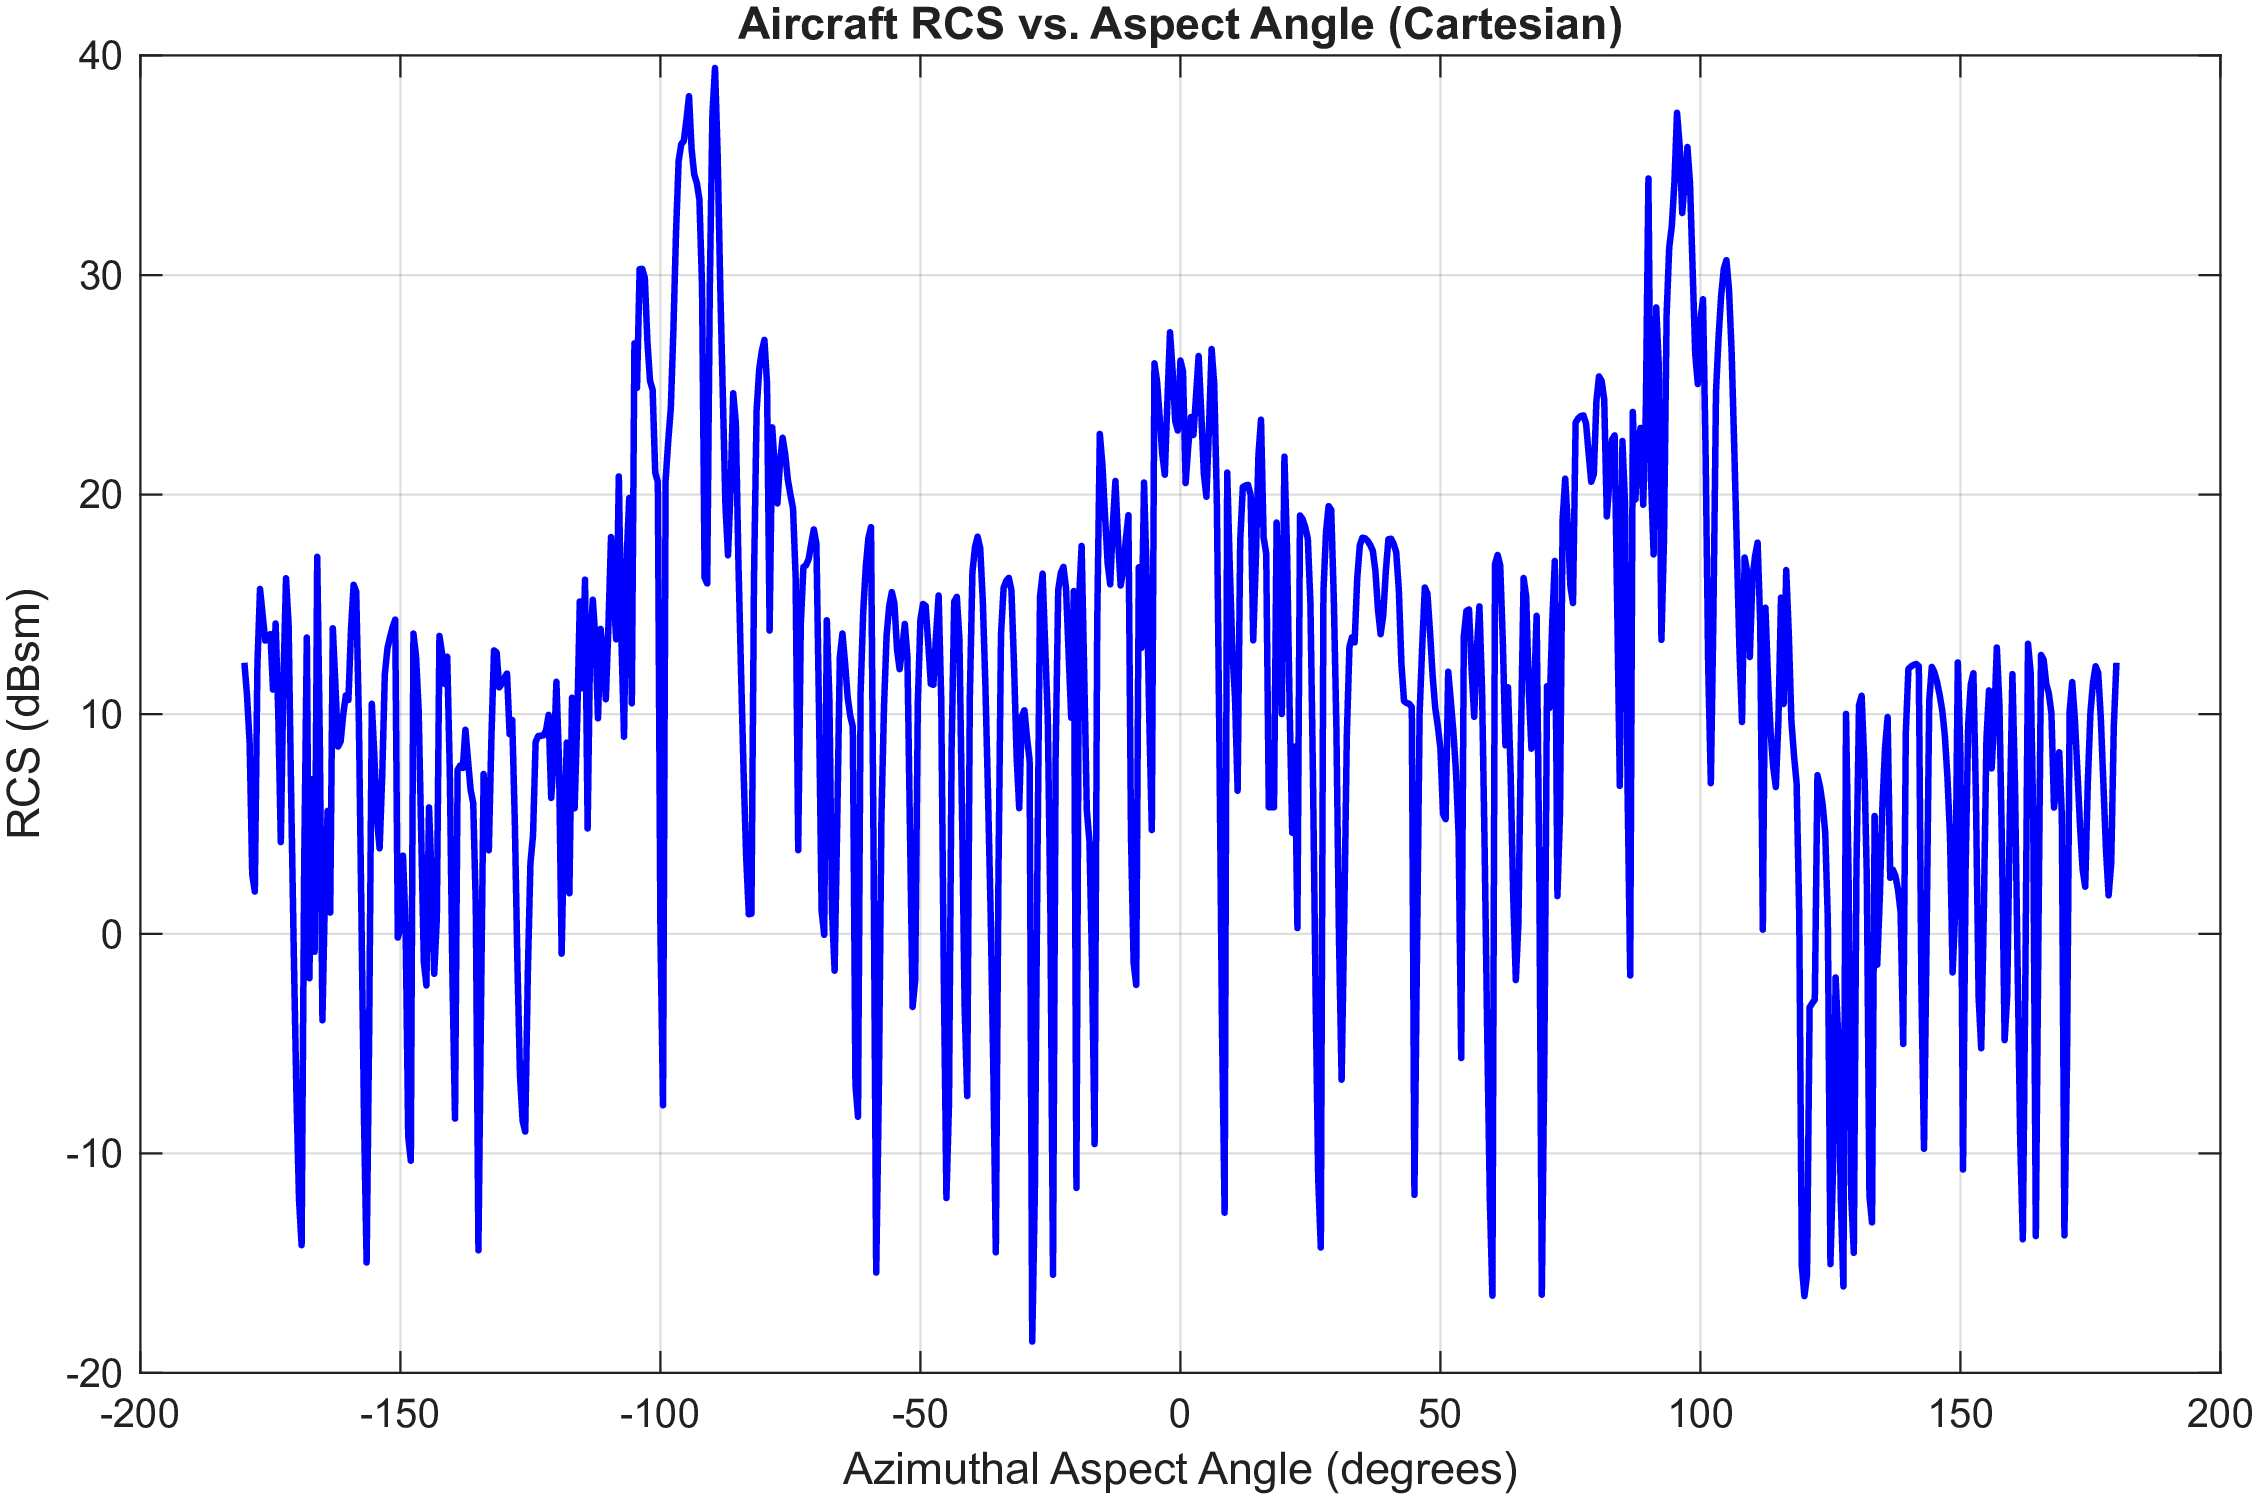
\includegraphics[width=8cm]{photos/project1_fig1.jpg}
    	\end{center}
    	\caption{Cartesian Coordinates RCS vs. Aspect Angle}
    	\label{Figure 1}
    \end{figure}
    \begin{figure}[H]
    	\begin{center}
    		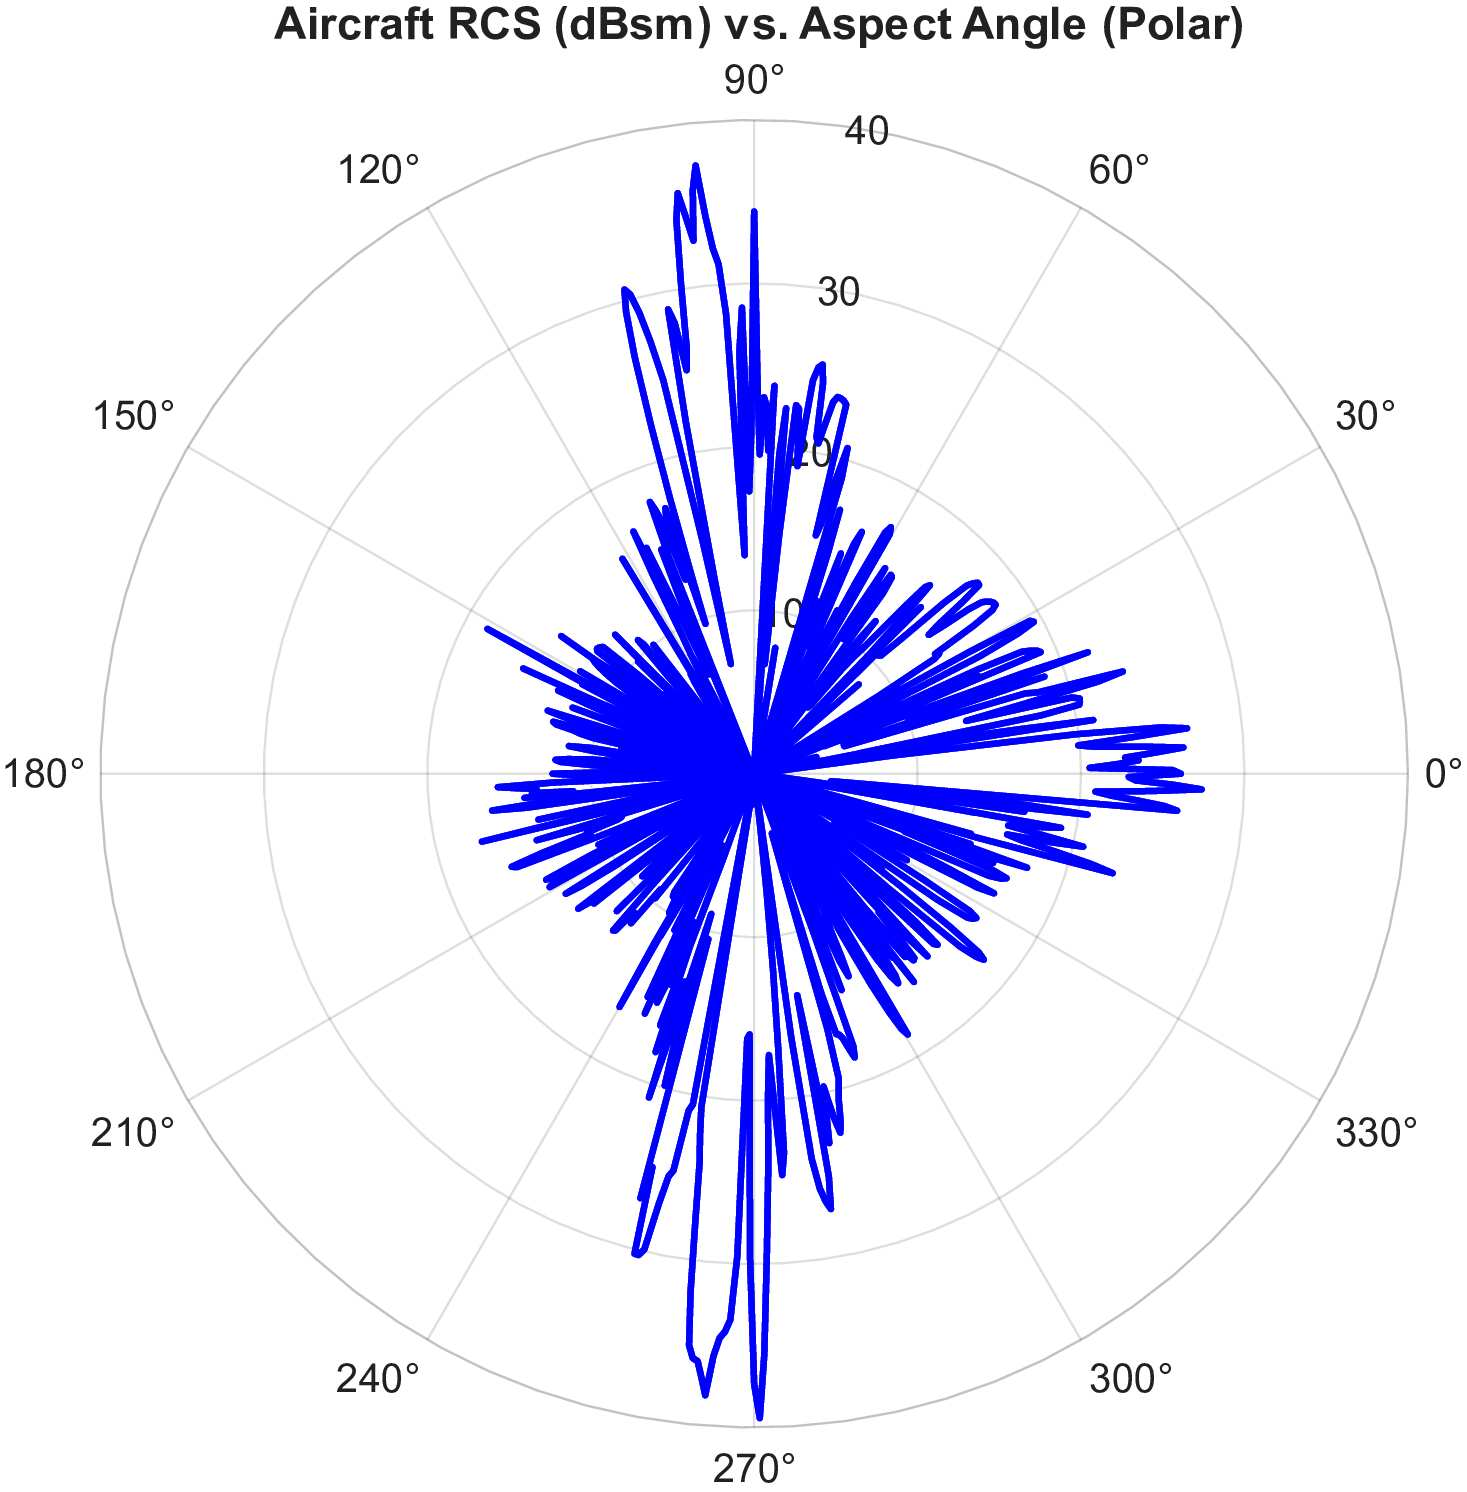
\includegraphics[width=7cm]{photos/project1_fig2.jpg}
    	\end{center}
    	\caption{Polar Coordinates RCS vs. Aspect Angle}
    	\label{Figure 2}
    \end{figure}
    
    The required gain $G_{req}$ plots in both Cartesian and Polar coordinates are created using Equation 3, and converted to decibels over isotropic using Equation 4. The polar coordinate version includes a dotted line indicating the 90 percent threshold, which indicates the overall antenna gain needed to cover 90 percent of the aspect angles. The plots are shown below:
    \begin{figure}[H]
    	\begin{center}
    		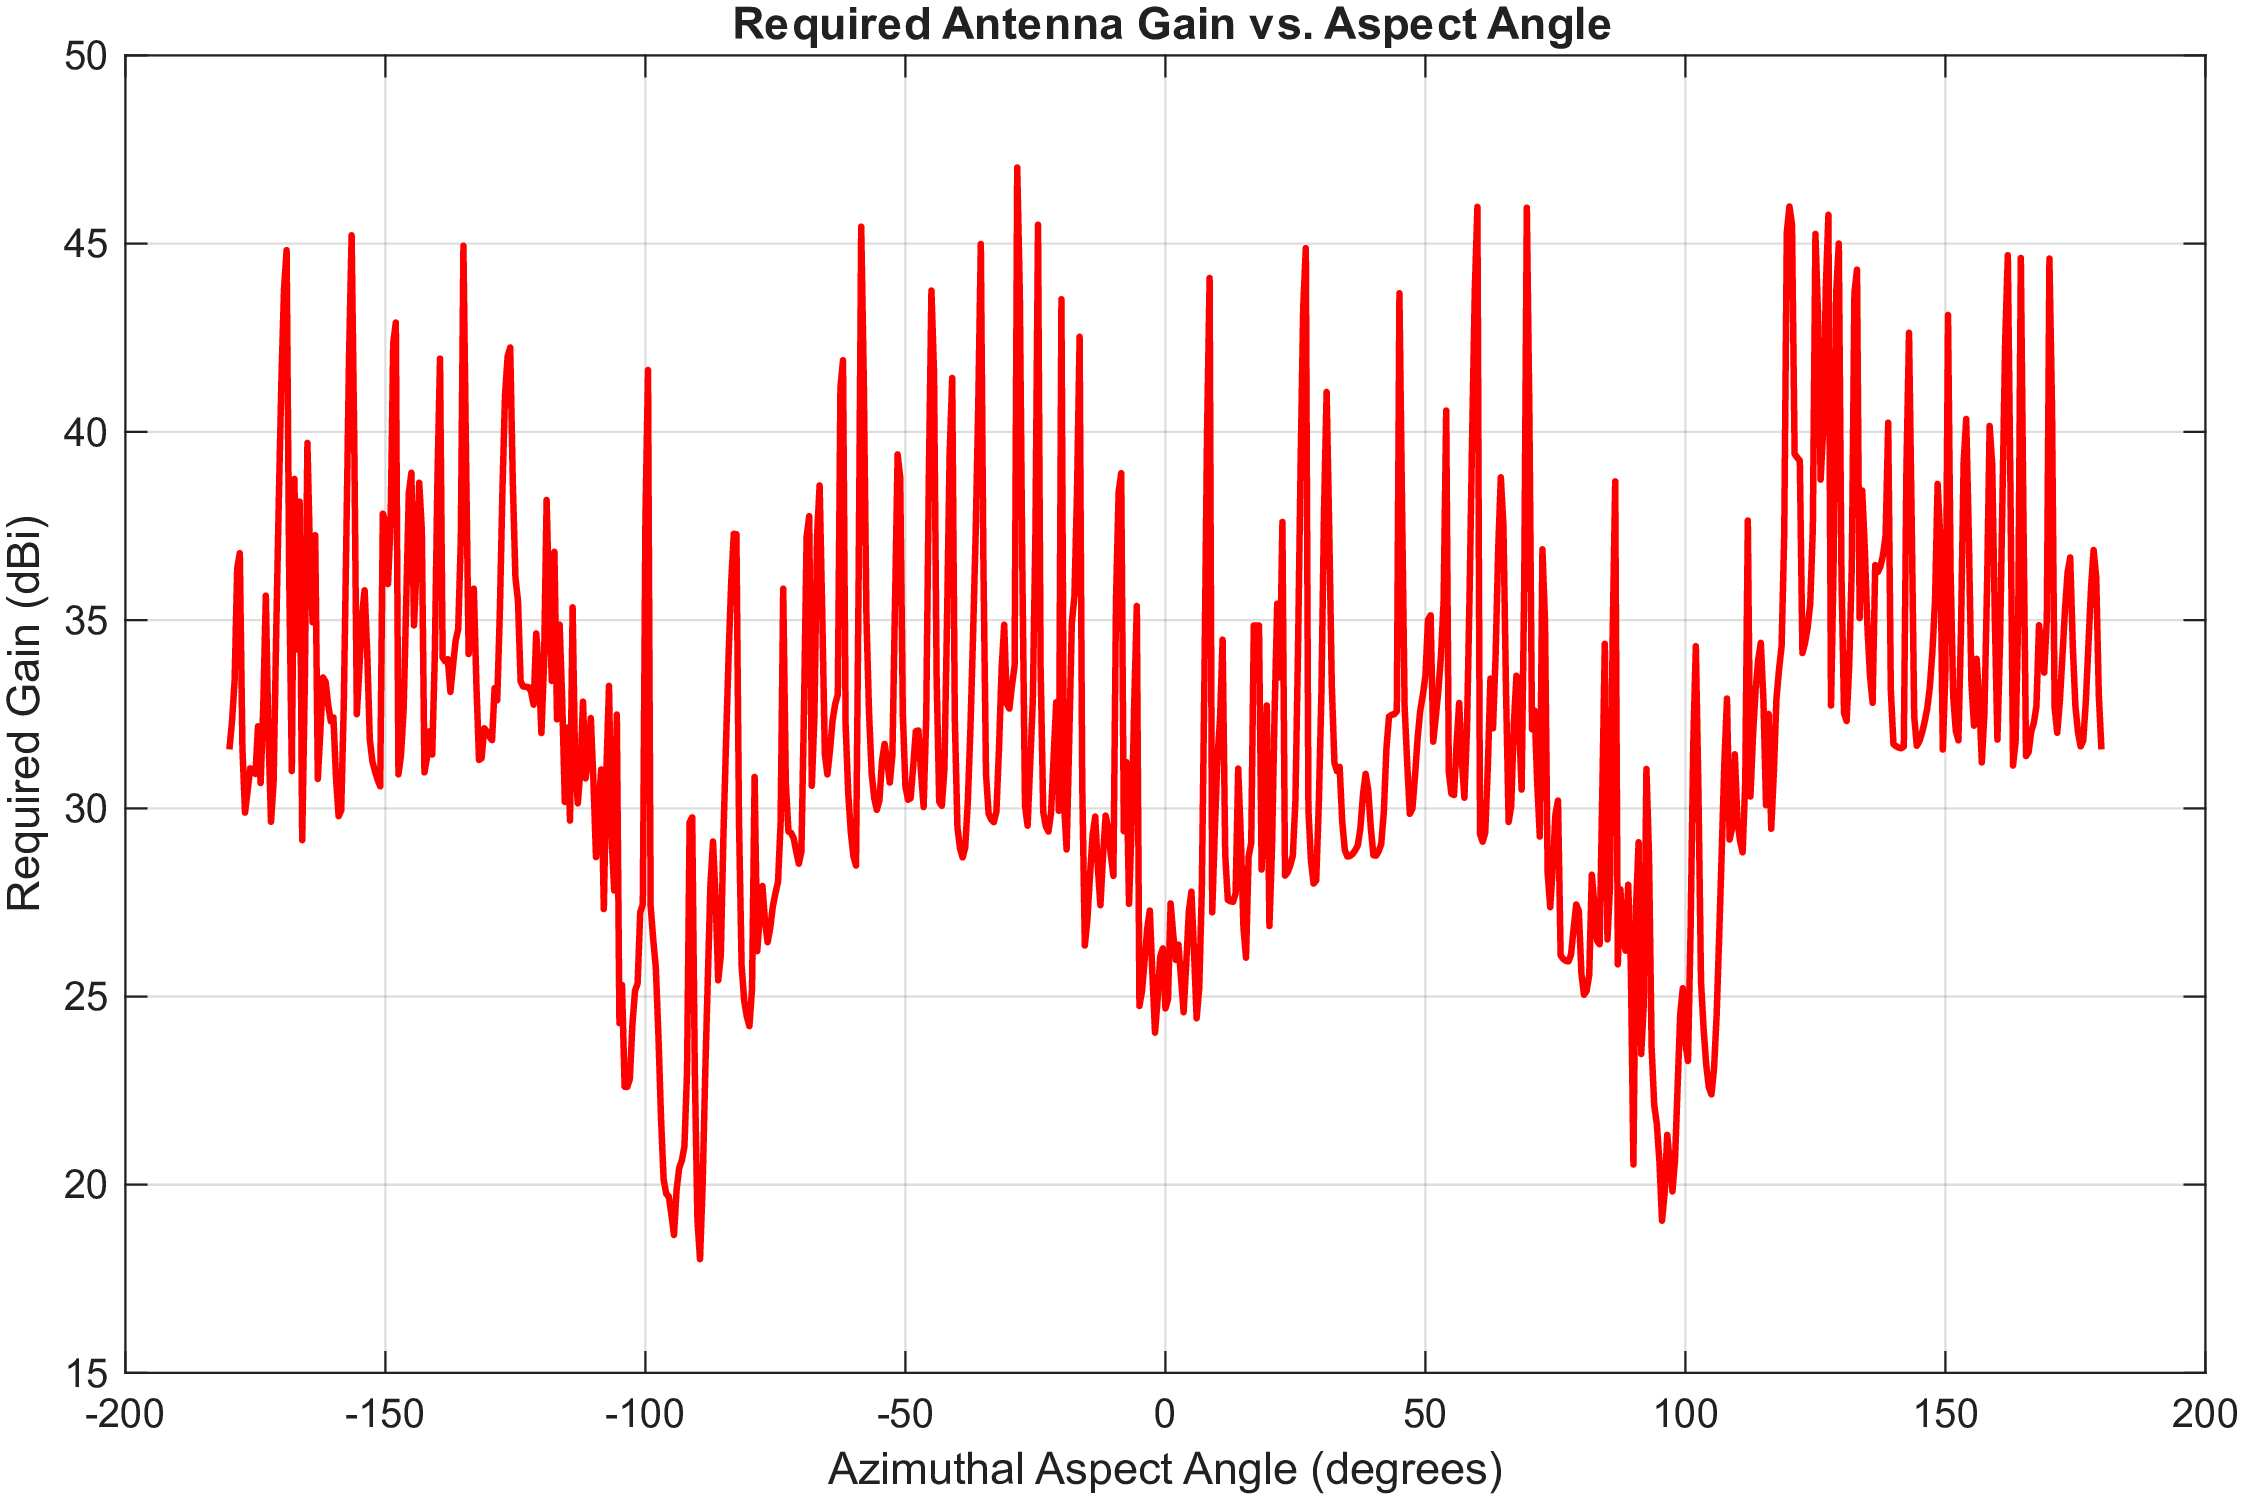
\includegraphics[width=10cm]{photos/project1_fig3.jpg}
    	\end{center}
    	\caption{Cartesian Coordinates Required Gain vs. Aspect Angle}
    	\label{Figure 3}
    \end{figure}
    \begin{figure}[H]
    	\begin{center}
    		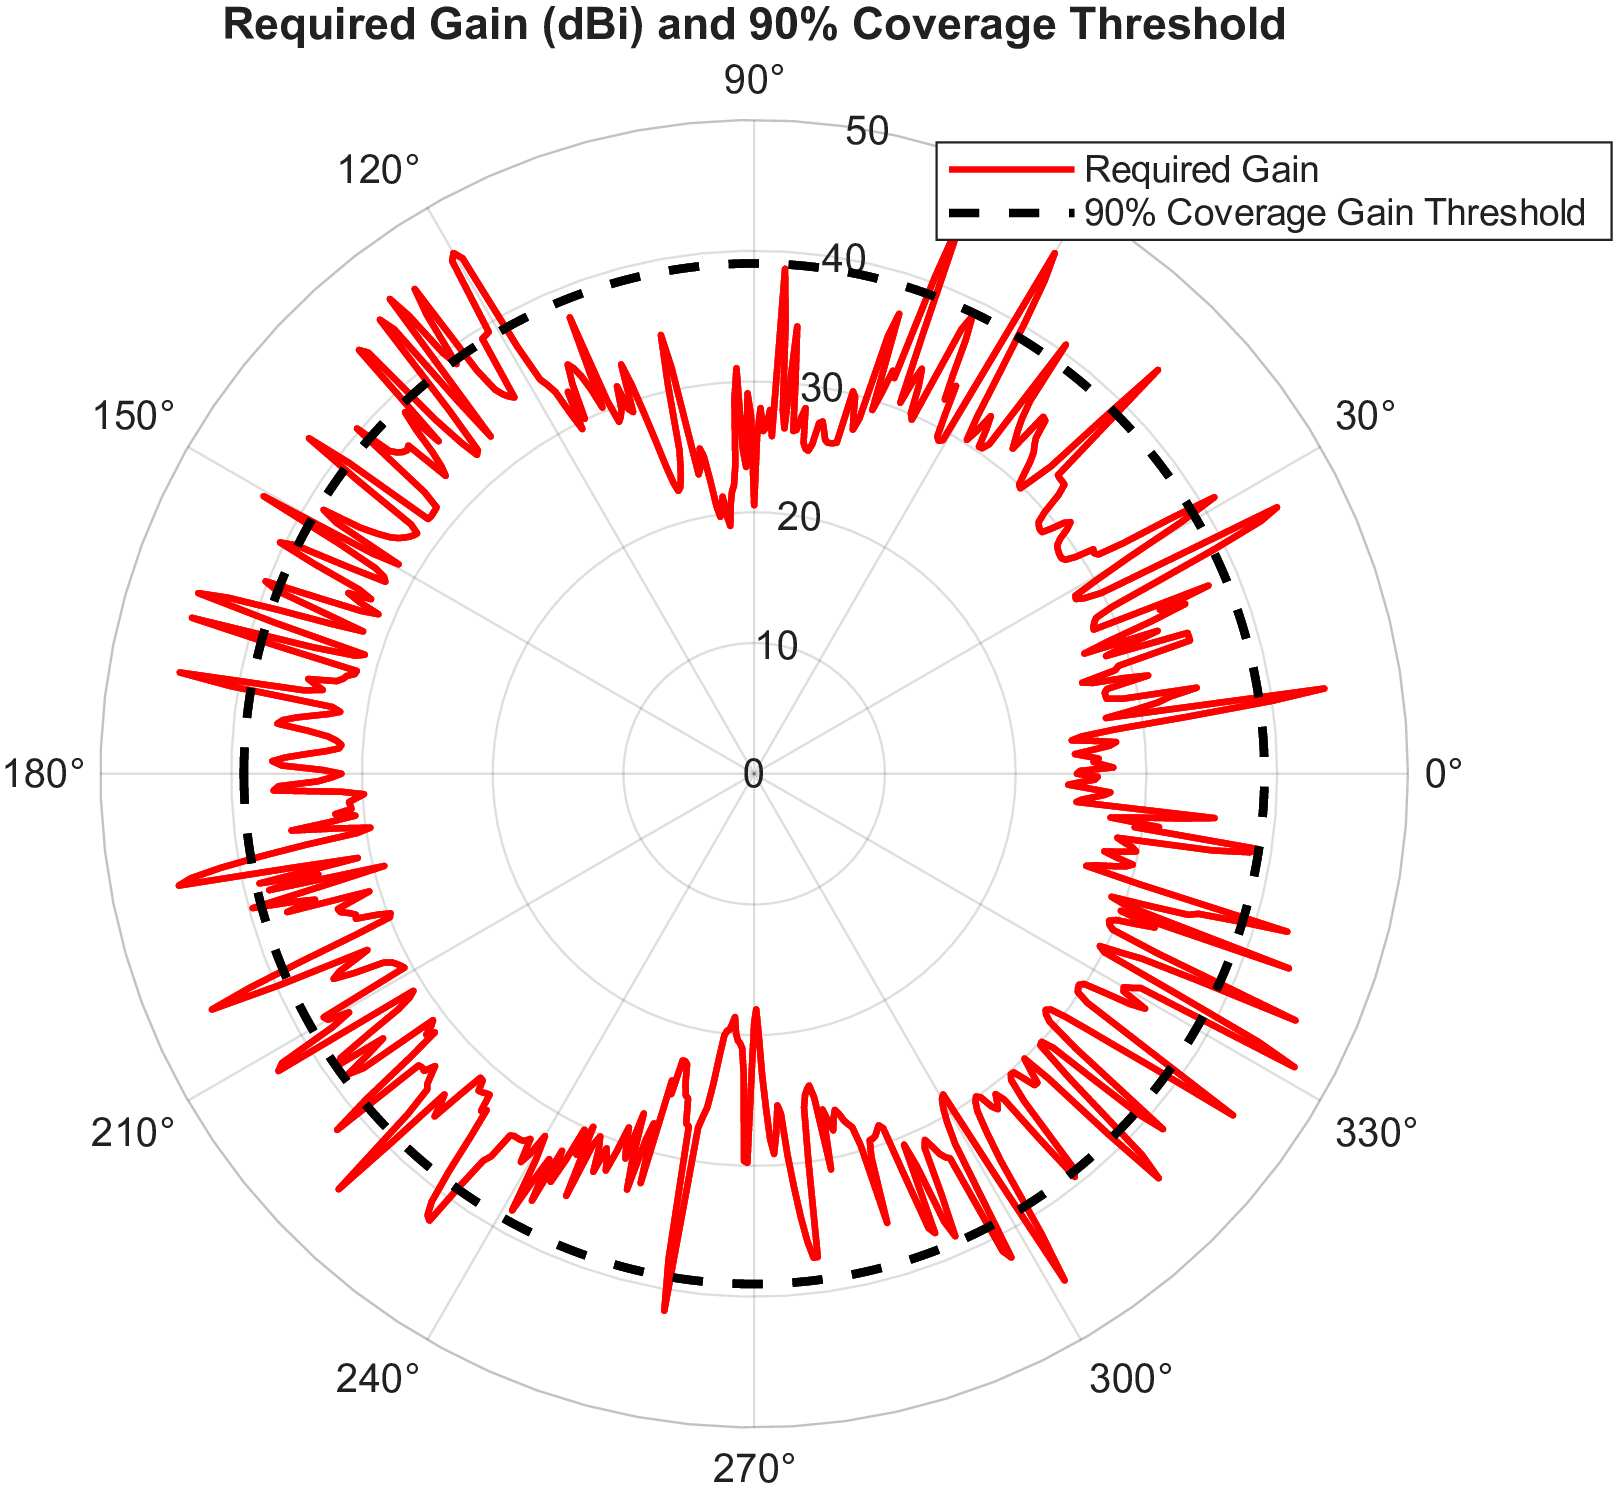
\includegraphics[width=10cm]{photos/project1_fig4.jpg}
    	\end{center}
    	\caption{Polar Coordinates Required Gain vs. Aspect Angle}
    	\label{Figure 4}
    \end{figure} 
    According to the polar plot, the required antenna gain $G$ equals 39.03 dBi, which when achieved should provide detection of the aircraft at $R_0 = 20$km for a minimum received power of $P_{rmin} = 1\cdot10^{-13}$W. Therefore, this gain will be utilized in our later calculations in order to determine our parabolic reflector antenna's physical parameters. \\\\
    
    Utilizing the required gain $G_{req} = 39.03$dBi for Equation 6, the parabolic reflector diameter, radius, and focal length (Assuming a focal ratio of $\frac{f_p}{D} = 0.35$) are calculated below:
    \begin{equation}
    	D = \frac{\lambda}{\pi} \sqrt{\frac{G_{req}}{\eta_{ap}}} = 1.464\text{m}
    \end{equation}
    \begin{equation}
    	a = \frac{D}{2} = 0.732\text{m}
    \end{equation}
    \begin{equation}
    	f_p = \frac{f_p}{D} \cdot D = 0.512\text{m}
    \end{equation}
    The parabolic reflector cross-section is sketched below, with the diameter, radius and focal length apparent from the plot. These parameters will be utilized in the MATLAB Antennas toolbox to design an antenna which attains the required gain $G_{req}$.
    \begin{figure}[H]
    	\begin{center}
    		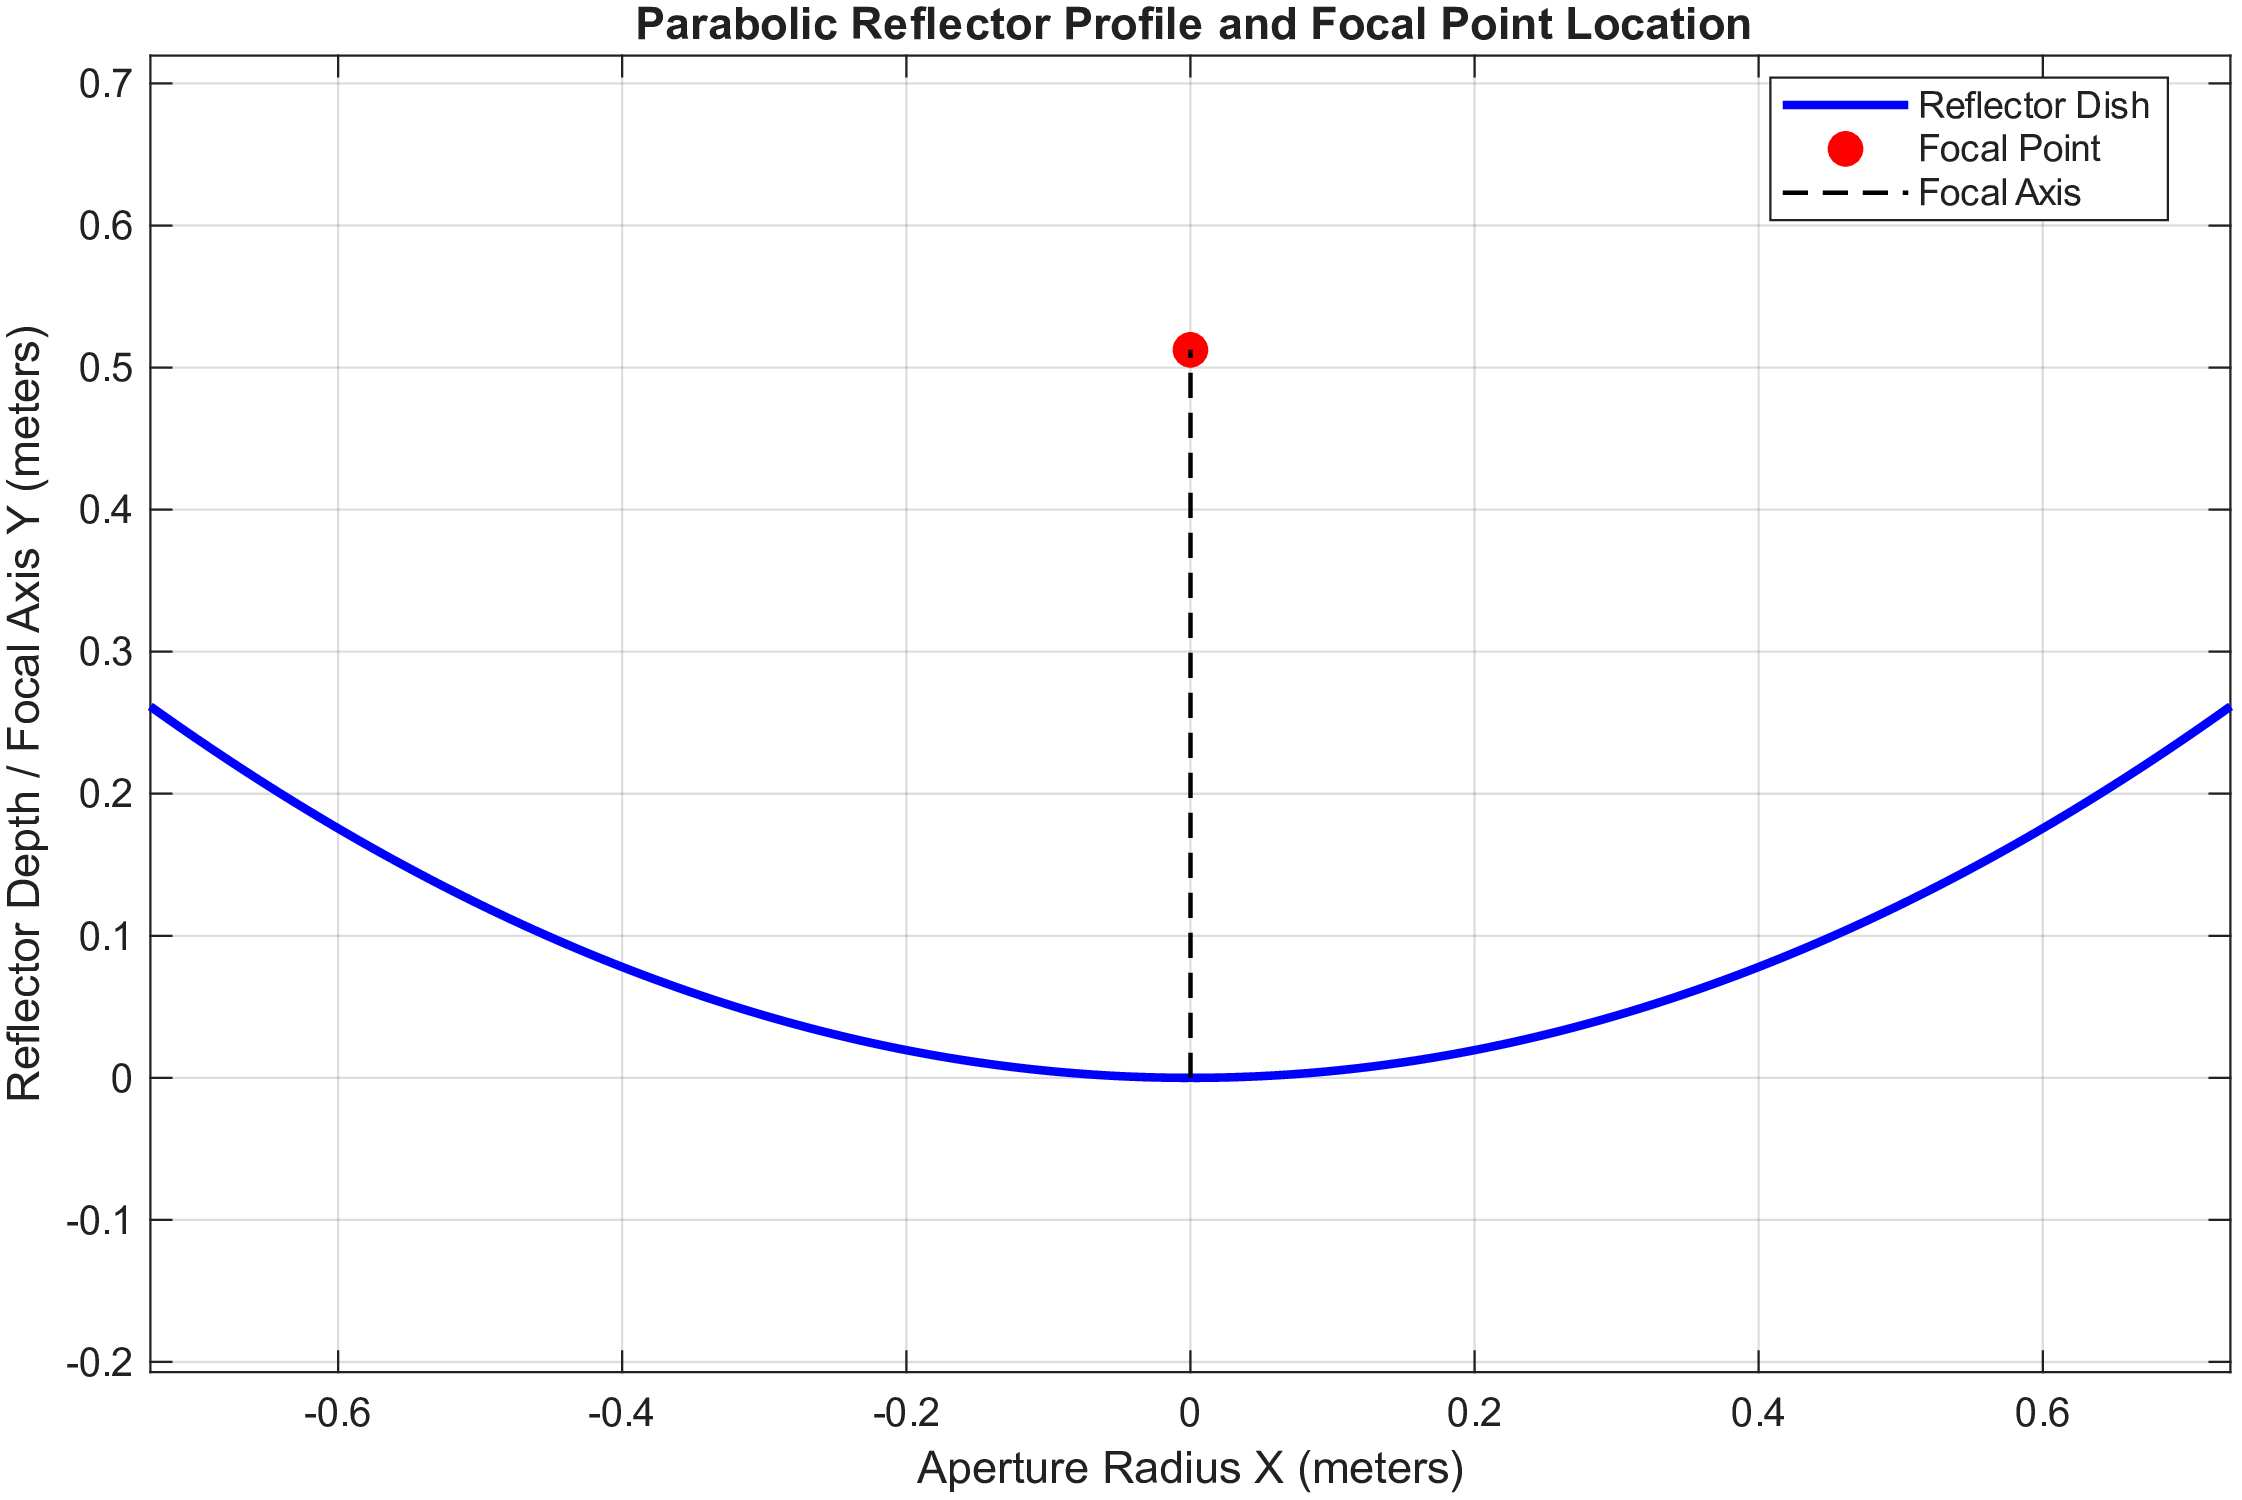
\includegraphics[width=13cm]{photos/project1_fig5.jpg}
    	\end{center}
    	\caption{Parabolic Reflector Sketch}
    	\label{Figure 5}
    \end{figure}
    
\section{Results}
	The MATLAB Antennas Toolbox is utilized to design an antenna which meets the required gain $G_{req}$ such that 90 percent aspect angle coverage is achieved. The required gain is given below for reference:
	\begin{equation}
		G_{req} = 39.03\text{dBi}
	\end{equation}
	
	A parabolic reflector antenna model is chosen from the Backing Structure options. The design frequency is chosen as $f = 10$GHz, and the calculated focal length $f_p$ and radius $a$ are input within the Properties section. The elevation pattern (EL Pattern) of directivity is used to determine if the antenna reaches the required gain $G_{req}$. The plot is shown below:
	\begin{figure}[H]
		\begin{center}
			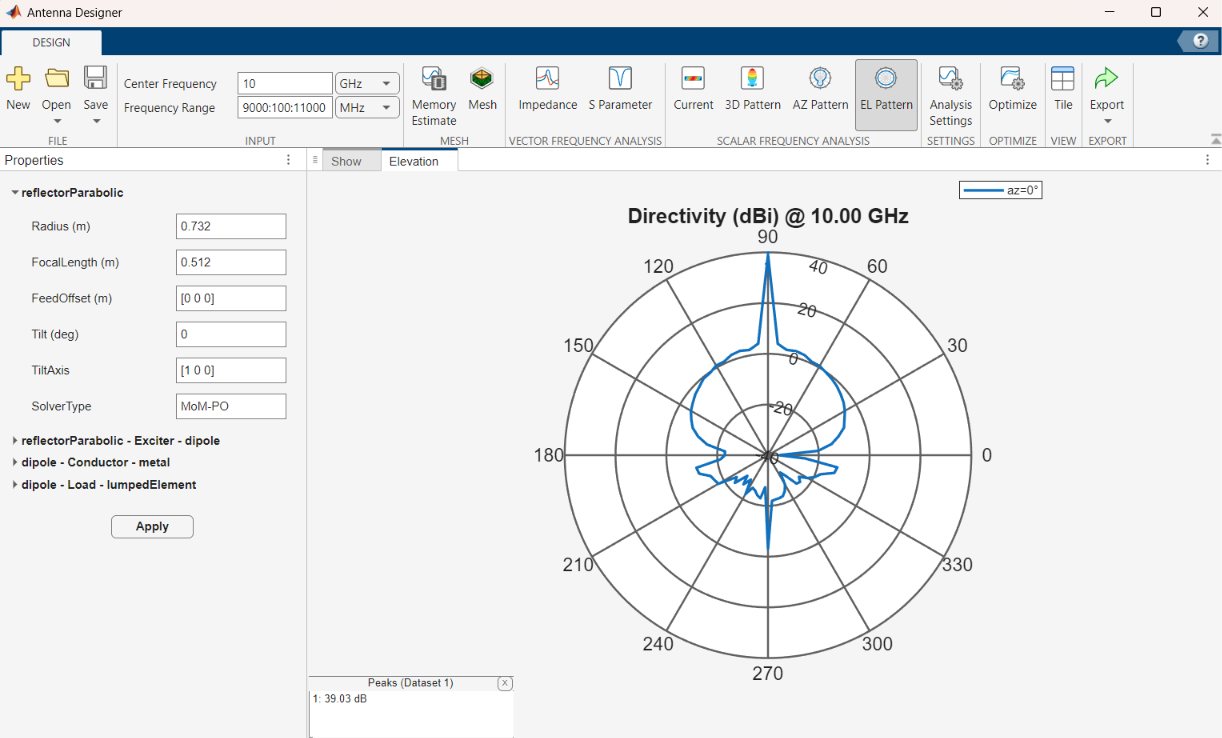
\includegraphics[width=14cm]{photos/project1_fig6.png}
		\end{center}
		\caption{Directivity of the Designed Parabolic Reflector Antenna}
		\label{Figure 7}
	\end{figure} 
	Clearly, the antenna gain hits a maximum of $39.03$dBi, which is exactly the gain required for our aircraft-radar system to work for an aspect angle coverage of 90 percent. Clearly, our design matches our calculations closely, and for this given design frequency; a parabolic reflector antenna with radius $a = 0.732$m and focal length $f_p = 0.512$m should meet the project requirements without issue.
	
	It is important to note that the feed-antenna is a dipole antenna by default, and results in aperture efficiency $\eta_{ap} = 0.34$. This is exactly the aperture efficiency utilized in our calculations, so this default setting is kept the same in order to achieve the proper results.
	
\section{Conclusions}
	All objectives defined above were achieved. This includes:
	\begin{itemize}
		\item Calculated the required gain $G_{req}$ such that 90 percent aspect angle coverage is achieved.
		\item Determine the diameter, radius and focal length of a parabolic reflector antenna which achieves the required gain.
		\item Design the parabolic reflector antenna to achieve the required gain for our aircraft-detection radar application in the MATLAB Antennas Toolbox.
		\item Include all plots described in the Aircraft-Detection Radar Requirements PDF. 
	\end{itemize}
	The parabolic reflector antenna design achieved the required gain $G_{req} = 39.03$dBi utilizing the calculated antenna radius and focal length, indicating that our theoretical calculations matched the real world properties of parabolic reflector antennas for our aircraft-detection radar application.
	
\section{References}
    Project 1: Aircraft-Detection Radar Requirements PDF \\
    ECGR 5121 Github Repo: Contains MATLAB code and RCS Excel data \\
    \url{https://github.com/Polaris-IPT/ECGR_5121}


\end{document}
